\documentclass[pdflatex,sn-vancouver-num]{sn-jnl}

\usepackage{graphicx}
\usepackage{geometry}
\usepackage{multirow}
\usepackage{amsmath,amssymb,amsfonts}
\usepackage{amsthm}
\usepackage{mathrsfs}
\usepackage[title]{appendix}
\usepackage{xcolor}
\usepackage{textcomp}
\usepackage{manyfoot}
\usepackage{booktabs}
\usepackage{algorithm}
\usepackage{algorithmicx}
\usepackage{algpseudocode}
\usepackage{listings}
\usepackage{wrapfig}
\usepackage{subcaption}
\usepackage{makecell}

\usepackage[colorlinks=true,linkcolor=blue,citecolor=blue,urlcolor=blue]{hyperref}

\graphicspath{{Figures/}}

\theoremstyle{thmstyleone}
\newtheorem{theorem}{Theorem}
\newtheorem{proposition}[theorem]{Proposition}

\theoremstyle{thmstyletwo}
\newtheorem{example}{Example}
\newtheorem{remark}{Remark}

\theoremstyle{thmstylethree}
\newtheorem{definition}{Definition}

\raggedbottom

\begin{document}

\title[Learning-to-Rank for Expedia Hotel Search]{A Notebook-Driven Learning-to-Rank Pipeline for the Expedia Personalised Hotel Search Task}

\author[1]{\fnm{Hidde} \sur{Franke (2840386)}}

\affil[1]{\orgdiv{Data Mining Techniques Group 5}, \orgname{VU Amsterdam}, \country{Netherlands}}

\abstract{The Expedia Personalised Hotel Searches dataset, introduced at ICDM 2013 and reused as the second assignment of the VU MSc Data Mining Techniques course, asks the model to order the candidate hotels of each search so that booked and clicked properties surface near the top. This report describes a fully reproducible pipeline that takes the raw five million row CSV files through exploration, cleaning, feature engineering, two-model hyperparameter tuning, locked-holdout evaluation, and a deployment-time fairness rerank. The feature set of 69 columns is motivated by published work on this dataset: 4 within-search relativisations following Wang and Kalousis, and 12 leakage-safe historical priors built with 5-fold out-of-fold target encoding following Bellucci et al. Both LightGBM LambdaRank and XGBoost \texttt{rank:ndcg} are tuned with 50 Optuna TPE trials on a locked validation slice. A weighted blend of the three-seed LightGBM ensemble and a single XGBoost model reaches NDCG@5 = 0.41521 on a 19{,}980-search locked holdout and NDCG@5 = 0.41706 on the Kaggle public leaderboard, slightly above the holdout estimate. A popularity-tertile audit reveals an exposure imbalance even though conditional NDCG@5 is in fact higher for the low-popularity tail; a val-tuned additive inference-time rerank lifts medium-tertile NDCG by 0.009 and exposure by 0.014 at a global NDCG cost of 0.0002.}

\keywords{Learning-to-rank, LambdaMART, Target encoding, Hyperparameter optimisation, Fairness of exposure}

\maketitle

\section{Introduction}\label{sec:introduction}
% !TEX root = ../main.tex

The Expedia Personalised Hotel Searches dataset originates from the ICDM 2013 competition of the same name and is reused for the in-class Kaggle competition of the VU MSc Data Mining Techniques course. Each row of the training and test files corresponds to one (search, property) pair, and the task is to rank the candidate hotels within each search query so that booked and clicked properties appear at the top. The course evaluates submissions with NDCG@5 under the IDCG = 0 convention, which scores searches with no positive labels as 0 rather than leaving them undefined. This convention has a direct impact on the headline number, because roughly half of the holdout searches contain no booking or click in the top five even at the model's best operating point.

The task fits the listwise learning-to-rank framing. LambdaMART, introduced by Burges~\cite{burges2010ranknet} as an extension of MART with a listwise gradient that approximates NDCG, is the natural model family and is also what the top-ranked entries of the 2013 competition used. Liu et al.~\cite{liu2013expedia} combined an ensemble of about thirty base learners, with LambdaMART carrying the largest weight, to reach the 1st-place private leaderboard score of NDCG@38 = 0.535. Wang and Kalousis~\cite{wang2014expedia} placed second with roughly 300 engineered features dominated by within-query relativisations of price and quality. More directly comparable to our setting, because the metric is NDCG@5 on the in-class leaderboard rather than NDCG@38 on the ICDM private set, is Bellucci et al.~\cite{bellucci2021dmt}, whose 2021 VU MSc Data Mining Techniques course report reported a public NDCG@5 of 0.41726 using LightGBM LambdaMART with leave-one-out (LOO) target encoding on \texttt{prop\_id} and a per-property positional proxy from rows where Expedia had shuffled the page (\texttt{random\_bool} = 1).

Our pipeline draws on this prior work but is otherwise built from scratch as six numbered notebooks. Three contributions are worth flagging up front. First, target encoding follows the Bellucci recipe but uses 5-fold out-of-fold (OOF) encoding rather than LOO; OOF is computationally cheaper at 4.96M rows and avoids the Bellucci variance at low-impression \texttt{prop\_id} values. Second, hyperparameter tuning uses Optuna's Tree-structured Parzen Estimator (TPE)~\cite{bergstra2011tpe,akiba2019optuna} on both LightGBM and XGBoost, with the LightGBM ensemble blended with XGBoost at a val-chosen weight. Third, a deployment-time fairness-of-exposure rerank, following the Singh and Joachims~\cite{singh2018fairness} framework, is added on top of the trained models and tuned on val with a pre-specified accuracy-fairness contract before being measured on the locked holdout.

The remainder is structured as follows. Section~\ref{sec:data} covers exploration, cleaning, and feature engineering. Section~\ref{sec:models} describes algorithm choice, Optuna tuning, the position-bias correction experiment, and the seeded ensemble plus LightGBM-XGBoost blend. Section~\ref{sec:eval} reports holdout NDCG@5 by predictor, by search-page size, and by ranked vs random page, together with a worst-case characterisation and feature importance. Section~\ref{sec:bias} presents the bias audit and the inference-time rerank. Section~\ref{sec:final} summarises the final pipeline and reports the realised Kaggle public score. Section~\ref{sec:disc} closes with a discussion that includes a short reflection on NDCG@5 versus alternative ranking metrics, limitations, and reproducibility.


\section{Data and Feature Engineering}\label{sec:data}
% !TEX root = ../main.tex

\subsection{Exploratory data analysis}

The training set contains 4{,}958{,}347 rows distributed over 199{,}795 unique search queries; the test set contains 4{,}959{,}183 rows over 199{,}549 searches. Every search returns between 5 and 38 candidate hotels with a sharp mode at 32, which corresponds to the default search-results page size on the Expedia website (see Fig.~\ref{fig:group-sizes}). Both train and test cover the period 2012-11-01 to 2013-06-30, so the partition is a random sample of search queries rather than a temporal split. This simplifies the use of historical priors, because no train search lies temporally before any test search; the priors aggregate the entire train slice without any look-ahead risk.

\begin{figure}[t]
\centering
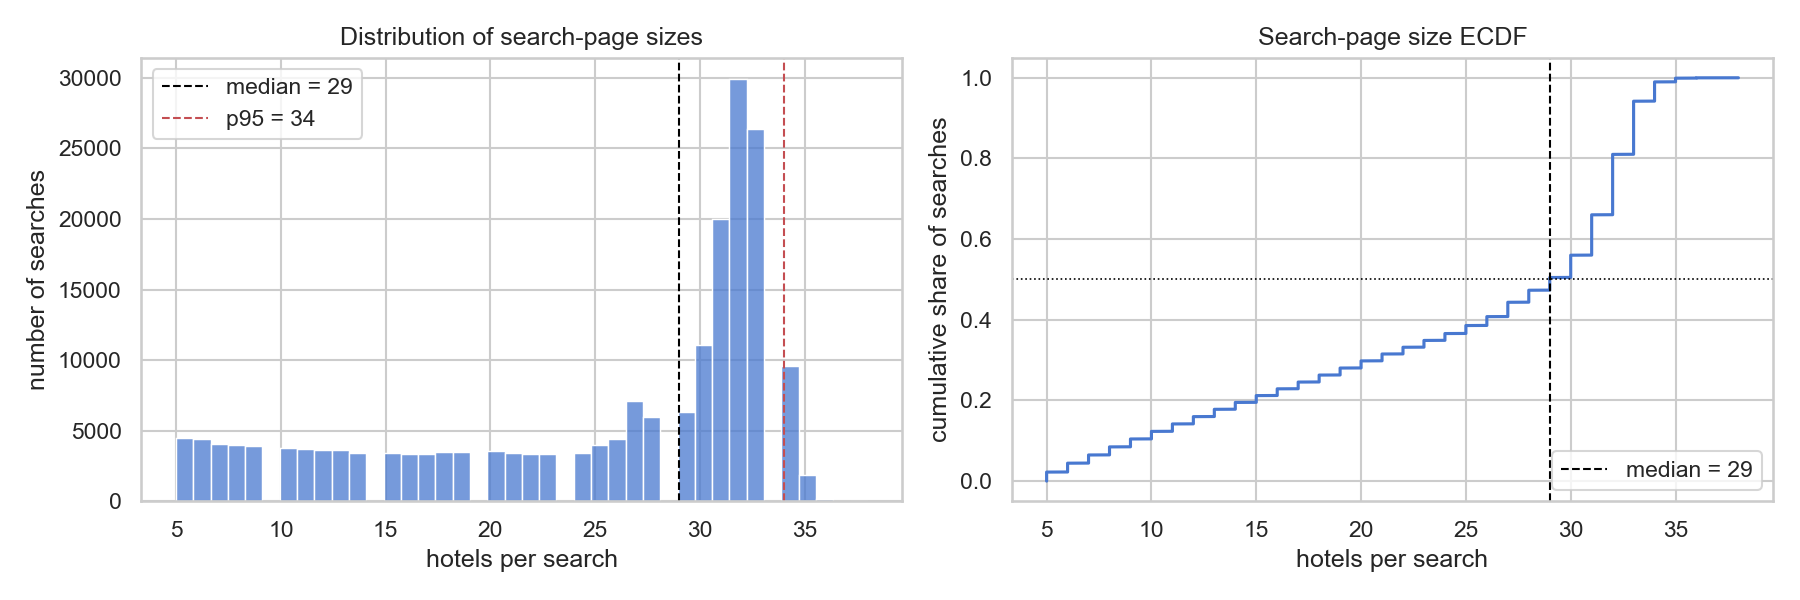
\includegraphics[width=0.95\linewidth]{eda_group_sizes.png}
\caption{Distribution of candidates per search. Left, histogram with the median at 29 hotels and the 95th percentile at 34. Right, empirical CDF; the distribution is roughly uniform between 5 and 29 candidates and then concentrates sharply around the default page size of 32.}
\label{fig:group-sizes}
\end{figure}

The relevance label is constructed as $\mathrm{rel} = 5 \cdot \mathbf{1}_{\mathrm{book}} + 1 \cdot \mathbf{1}_{\mathrm{click\,only}}$, giving label counts $\{0: 4{,}736{,}468,\ 1: 83{,}489,\ 5: 138{,}390\}$ on the training set. About 95.5\% of rows carry no positive signal at all, which is typical for click-through ranking; a model must learn within-query contrasts rather than pointwise probabilities. The conditional rate $P(\text{book} \mid \text{click}) = 0.62$ shows that the click and book events are tightly coupled in the data and that treating booking and click as two separate sub-targets would be redundant.

Missingness clusters in three groups (Fig.~\ref{fig:missing}). The eight competitor blocks \texttt{comp1\_*} to \texttt{comp8\_*} are 83\% to 98\% missing because they are only filled when a competing online travel agent had a quote available. The two visitor-history columns (\texttt{visitor\_hist\_starrating} and \texttt{visitor\_hist\_adr\_usd}) are 95\% missing, reflecting first-time Expedia visitors. The query-affinity score \texttt{srch\_query\_affinity\_score} and the origin-distance column \texttt{orig\_destination\_distance} are 90\% and 32\% missing respectively. Crucially, LightGBM splits on missingness as a separate value rather than treating NaN as zero, so the missingness pattern itself becomes signal during training; we therefore preserve NaNs rather than impute them.

\begin{figure}[t]
\centering
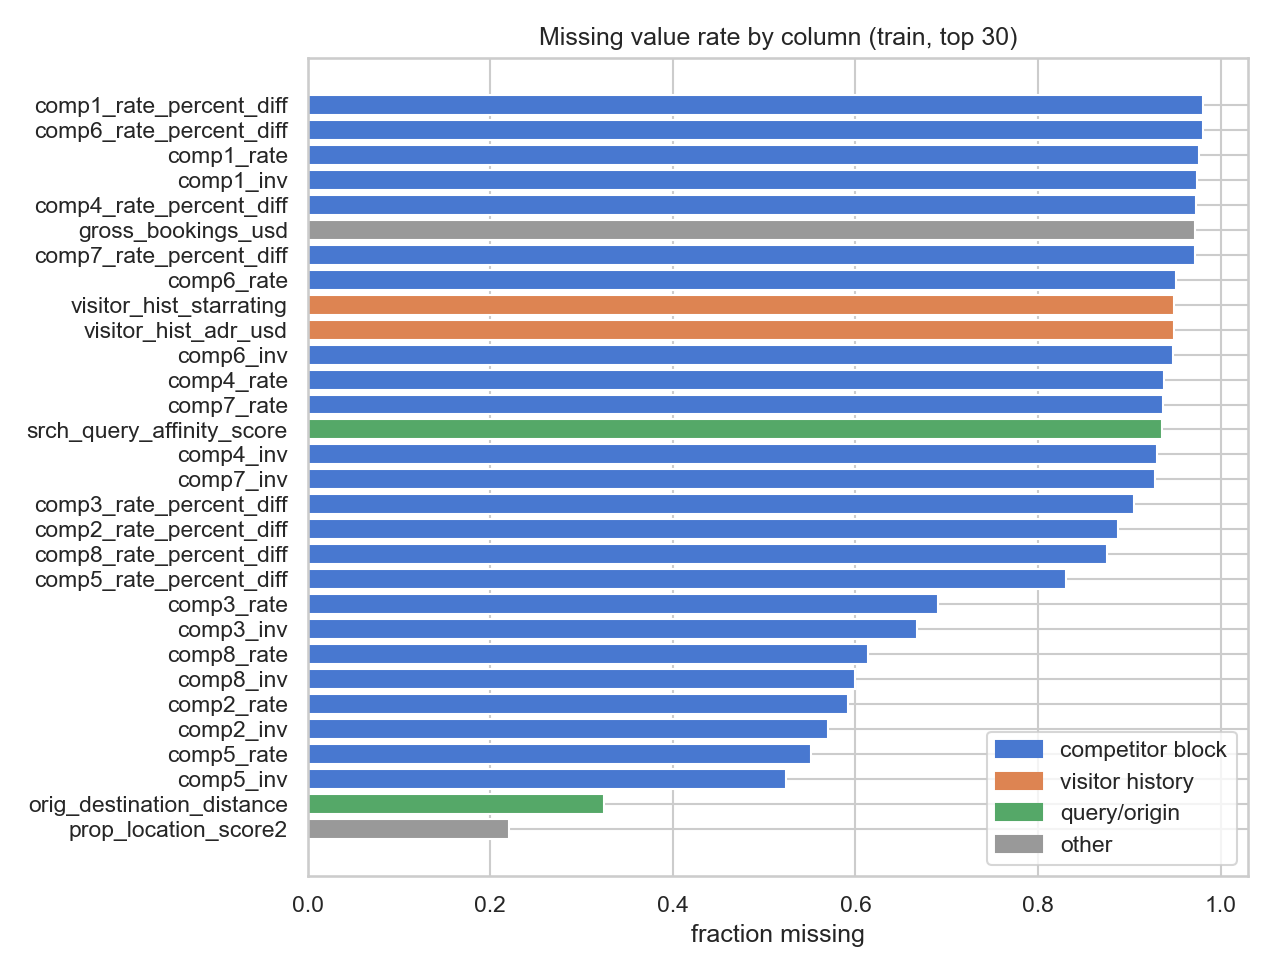
\includegraphics[width=0.95\linewidth]{eda_missingness.png}
\caption{Per-column missingness rate, sorted within four groups (raw numeric, visitor history, search-affinity, competitor block). The competitor block dominates the right tail; only \texttt{has\_visitor\_history} replaces these columns with a binary indicator.}
\label{fig:missing}
\end{figure}

The \texttt{price\_usd} column contains extreme outliers, with a maximum of USD 19.7 million on the full 4.96M-row training set. A $\log(1+x)$ transform compresses the range to roughly $[0, 16.8]$, which is friendly for any later arithmetic (within-search z-scores, deltas against \texttt{prop\_log\_historical\_price}, and ratios). We do not winsorise or clip; the choice of price transformation is made on the basis of an early ablation against the within-search relativisations described in Section~\ref{subsec:feat}.

Categorical cardinality matters for encoding decisions. Small-cardinality columns (\texttt{site\_id} = 34 unique values, country IDs around 200) are passed as native LightGBM categoricals and admit straightforward one-hot encoding for XGBoost via the DMatrix categorical conversion. Large-cardinality columns (\texttt{prop\_id} with 129{,}113 unique values, \texttt{srch\_destination\_id} with 18{,}127) cannot reasonably be one-hot encoded; we pass them as LightGBM native categoricals and rely on the historical priors of Section~\ref{subsec:feat} to carry their information into XGBoost. Coverage of the test categoricals by the train slice is high (99.7\% on \texttt{prop\_id}, 97.1\% on \texttt{srch\_destination\_id}), so the global-fallback branch of the target encoder rarely fires on test.

Spearman correlations against the booking indicator (Fig.~\ref{fig:corr}) confirm two structural facts of this dataset. First, raw \texttt{price\_usd} carries essentially zero global correlation with booking ($\rho = -0.0001$): without context an absolute price tells the model nothing, because prices vary by city and currency. The same property in a different city has the same \texttt{price\_usd} but a completely different position in the user's choice set. Second, within-query relativisations of price and quality (Section~\ref{subsec:feat}) reach correlations around $0.10$ to $0.13$ with booking and $0.20$ to $0.25$ with the composite relevance grade, more than two orders of magnitude above the raw price.

\begin{figure}[t]
\centering
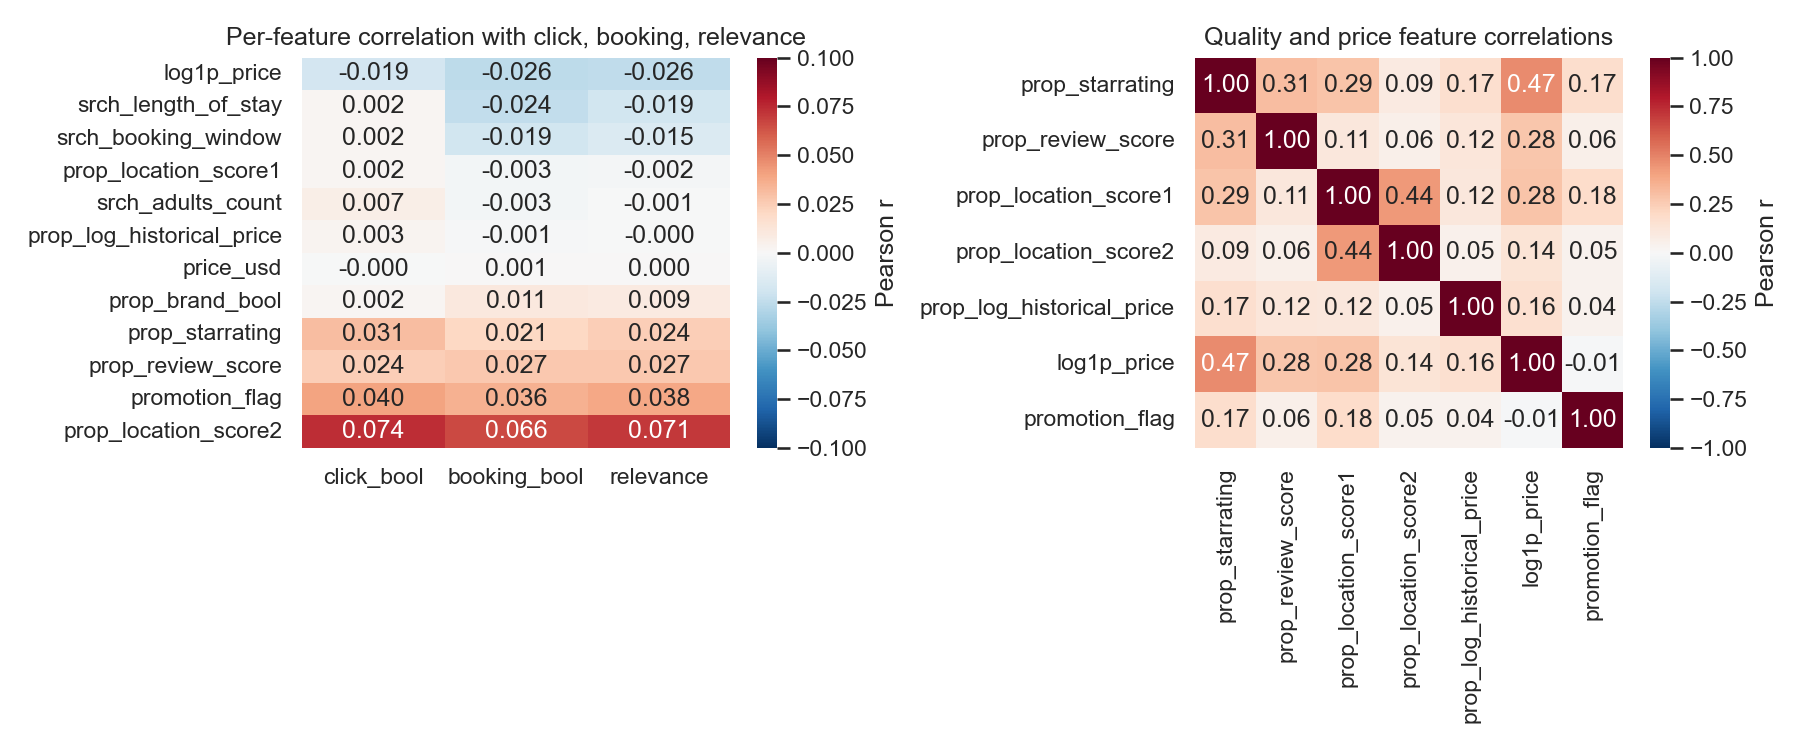
\includegraphics[width=0.95\linewidth]{eda_corr_booking.png}
\caption{Left, top-20 features by absolute Spearman correlation against the booking indicator on the 4.96M-row train set. Within-search relativisations and historical priors dominate the raw columns. Right, inter-correlation among the eight strongest quality features; \texttt{prop\_location\_score2} carries unique signal not redundant with price or star rating.}
\label{fig:corr}
\end{figure}

\subsection{Cleaning}

Data cleaning is deliberately conservative because LightGBM handles missing values natively and any imputation would discard the missingness signal. Five lightweight transformations are applied to both train and test. First, \texttt{date\_time} is parsed into a real timestamp so that later derivations (month, weekday, hour) can be computed without re-parsing, although they did not end up in the final feature set. Second, a binary \texttt{has\_visitor\_history} flag is added, which equals 1 if either visitor-history column is non-null. The flag has rate 5.10\% on train and 5.13\% on test, consistent. Third, \texttt{log1p\_price} is added alongside the raw \texttt{price\_usd} (Fig.~\ref{fig:price}). Fourth, three cheap competitor aggregates are computed from the row's own 24 competitor columns: \texttt{comp\_count\_quoted} (number of non-null competitor rates), \texttt{comp\_pdiff\_mean}, and \texttt{comp\_rate\_mean}. None of these aggregates cross row boundaries, so they are leakage-free by construction. Fifth, type downcasting collapses \texttt{int64} to \texttt{int32} and \texttt{float64} to \texttt{float32}, reducing the in-memory footprint from 1.72 GB to 1.16 GB on train and from 1.56 GB to 1.08 GB on test, with no measurable precision loss for tree splits.

\begin{figure}[t]
\centering
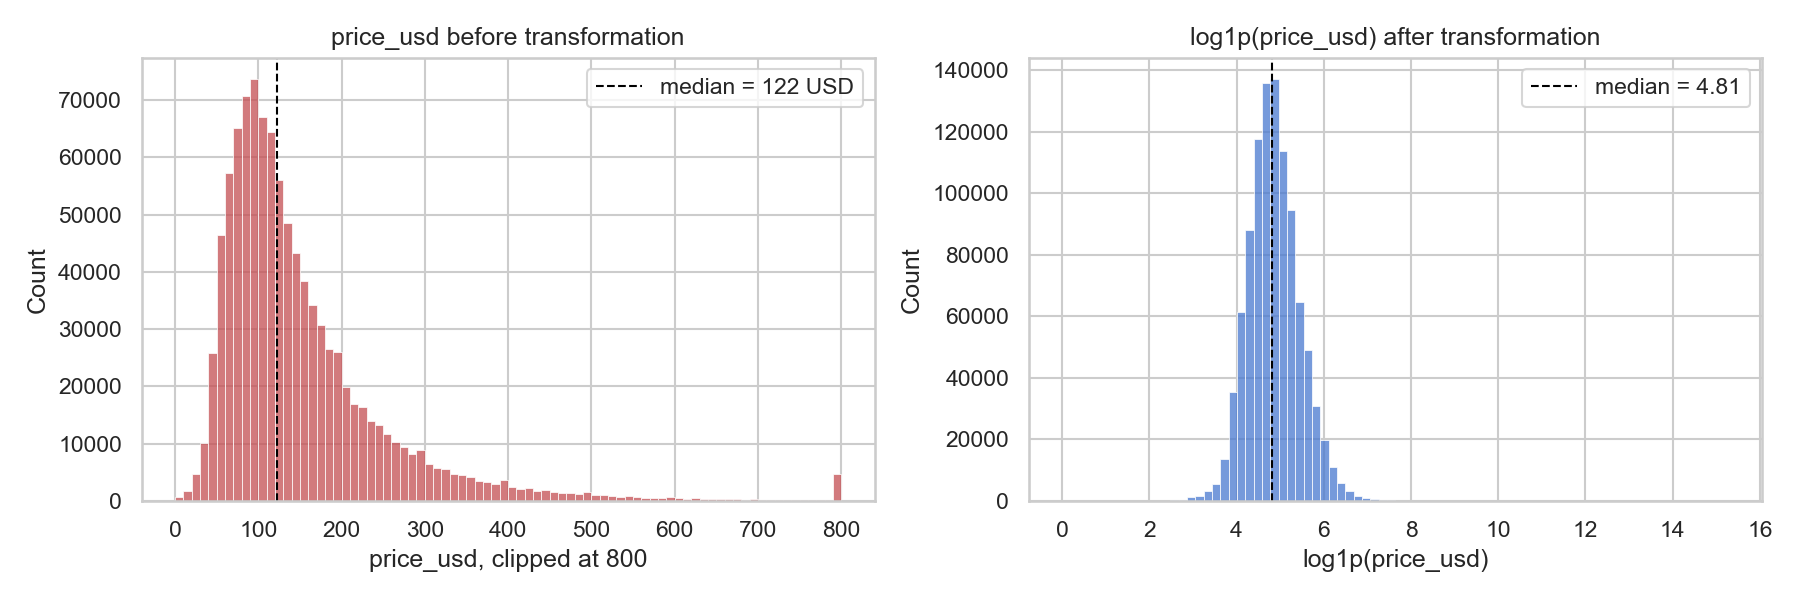
\includegraphics[width=0.85\linewidth]{cleaning_price_log_transform.png}
\caption{Price distribution before (left, clipped at USD 800 for visibility, median 122 USD) and after (right) the log1p transform (median 4.81). The original distribution has a heavy right tail up to USD 19.7 million; the log scale compresses it to a model-friendly $[0, 16.8]$ range.}
\label{fig:price}
\end{figure}

Three transformations are deliberately not applied. We do not impute competitor or visitor-history NaNs, because LightGBM splits on missingness as a separate value and that information is more useful intact. We do not winsorise \texttt{price\_usd}, because the choice of transformation depends on the downstream feature mix and the log transform is sufficient at this level. We do not encode categoricals at the cleaning stage; encoding is a feature-engineering choice that belongs in the next notebook.

\subsection{Feature engineering}\label{subsec:feat}

The locked train/val/holdout split is a group-aware 80/10/10 partition on \texttt{srch\_id} with seed 42, written to \texttt{split\_seed42.json} and reused by every later notebook. The split assigns 159{,}836 train searches (3{,}966{,}833 rows), 19{,}979 val (496{,}491 rows), and 19{,}980 holdout (495{,}023 rows). The holdout is locked: it never appears in feature engineering, training, hyperparameter selection, or fairness-rerank tuning. The val slice is used as the model-selection surface for Optuna trials, the blend weight, and the rerank lambda.

The feature set follows the published prior work on this dataset directly. The feature blocks are organised so that each is motivated by a specific reference and is added on top of the previous one only if it beats the previous on val NDCG@5 at the same anchor hyperparameters. Table~\ref{tab:fe} reports the trajectory.

\begin{table}[t]
\centering
\caption{Feature engineering ablation under a fixed LightGBM LambdaRank configuration (Bellucci~\cite{bellucci2021dmt} Table 3, 500 trees with early stopping on val NDCG@5). The hyperparameter sweep happens in Section~\ref{sec:models}.}
\label{tab:fe}
\begin{tabular}{lccc}
\toprule
Feature block & \# features & Best iter & Val NDCG@5 \\
\midrule
A: 53 raw + competitor block + categoricals & 53 & 407 & 0.39524 \\
B: + 4 within-search relativisations (Wang \& Kalousis) & 57 & 258 & 0.39884 \\
C: + 4 \texttt{prop\_id} OOF priors (Bellucci) & 61 & 263 & 0.40111 \\
D: + 4 \texttt{srch\_destination\_id} OOF priors & 65 & 378 & 0.40250 \\
E: + 4 (\texttt{prop\_id}, \texttt{srch\_destination\_id}) pair priors & 69 & 317 & 0.40258 \\
\bottomrule
\end{tabular}
\end{table}

Block B reflects the central insight of Wang and Kalousis~\cite{wang2014expedia}: ranking is an intra-query problem and absolute features matter less than their position relative to the other candidates in the same search. We add the per-search rank of \texttt{price\_usd}, the per-search z-score of \texttt{log1p\_price}, and the per-search deltas of \texttt{prop\_starrating} and \texttt{prop\_location\_score2}. These four features cost +0.00360 NDCG@5 over the raw baseline and reduce best-iteration from 407 to 258, indicating that the model converges faster when the within-query signal is exposed explicitly rather than learned implicitly.

Blocks C, D, and E implement leakage-safe historical priors following the Bellucci~\cite{bellucci2021dmt} target-encoding recipe, modified for tractability at 4.96M rows. We replace LOO encoding with 5-fold OOF encoding on \texttt{srch\_id} groups: each train row in fold $f$ receives priors aggregated over the other four folds, so its own click and book labels never enter its own prior. Validation, holdout, and test rows receive priors aggregated over the entire train slice. Smoothing follows the Laplace form $\widehat{r}_{\text{smooth}} = (\sum y + \alpha \bar y) / (n + \alpha)$ with $\alpha = 20$; unseen keys back off to the global rate. Per key we compute four statistics: log impressions, smoothed click rate, smoothed booking rate, and smoothed mean relevance. The \texttt{prop\_id} block contributes the largest single jump (+0.00227); the destination block adds a smaller +0.00139; the pair block contributes only +0.00008 in our setting, which is much less than what the autoresearch reference for this dataset would suggest. A plausible explanation is that block B already absorbs part of the within-search signal that the pair priors would otherwise carry.

Two further design choices, considered but not adopted, deserve a sentence. First, negative-row downsampling. Bellucci~\cite{bellucci2021dmt} explicitly tested downsampling negatives and reported overfitting, so they kept all rows. A small pilot at a 1:4 negatives-per-positive ratio confirms a 0.006 NDCG@5 drop on this dataset; the recipe transfers. Second, the per-property mean-position proxy from \texttt{random\_bool} = 1 rows, used by Bellucci, relies on the assumption that those impressions are position-uniform. On this dataset the position-by-\texttt{random\_bool} distribution is in fact decreasing rather than uniform, so the assumption underlying the proxy does not hold; the gain is below noise and the feature is not added.


\section{Models, Tuning, and Blend}\label{sec:models}
% !TEX root = ../main.tex

\subsection{Algorithm choice}

The two models are LightGBM LambdaRank~\cite{ke2017lightgbm} and XGBoost \texttt{rank:ndcg}~\cite{chen2016xgboost}. Both are gradient-boosted decision tree implementations of pairwise / listwise ranking objectives, but they differ in two substantive ways: LightGBM uses histogram-based split finding with native categorical support and a leaf-wise tree growth strategy, while XGBoost uses level-wise growth with a regularised objective and approximate split finding. The two implementations therefore explore the feature space along noticeably different trajectories. Liu et al.~\cite{liu2013expedia} made the same diversity argument when justifying their thirty-base-learner ensemble: ensemble lift comes from disagreement, and two implementations of roughly the same ranking idea disagree enough to be worth blending. The rubric of the in-class assignment also asks for two distinct techniques to be compared; LightGBM and XGBoost meet this requirement while keeping the implementation effort manageable.

\subsection{Hyperparameter optimisation with Optuna TPE}

We use Optuna's TPE sampler~\cite{bergstra2011tpe,akiba2019optuna} on each model independently, with 50 trials per model and val NDCG@5 as the objective. The TPE sampler fits a probabilistic surrogate over the search space after a 10-trial random warmup and then concentrates subsequent trials in regions of high estimated NDCG. The choice over a single-axis manual grid is twofold: TPE finds non-obvious parameter interactions that a univariate sweep misses, and it amortises tuning effort across both models with one consistent protocol. Each trial fits up to 1000 trees with early stopping at 30 rounds on val NDCG@5. The seed is fixed at 42, the studies are deterministic, and the holdout is untouched.

\begin{table}[t]
\centering
\caption{Hyperparameter search spaces and Optuna-selected values for LightGBM LambdaRank and XGBoost \texttt{rank:ndcg}. Best trial val NDCG@5 in the LightGBM study reaches 0.40999 at 423 trees; XGBoost reaches 0.41223 in the refit (Section~\ref{subsec:ensemble}) at 694 boosting rounds.}
\label{tab:hyper}
\begin{tabular}{lll}
\toprule
\multicolumn{3}{l}{\textbf{LightGBM LambdaRank}} \\
\midrule
Hyperparameter & Search space & Selected \\
\midrule
learning\_rate & loguniform [0.01, 0.10] & 0.0565 \\
num\_leaves & int [15, 127] & 110 \\
max\_depth & int [4, 12] & 7 \\
min\_child\_samples & int [10, 200] & 74 \\
bagging\_fraction & uniform [0.5, 1.0] & 0.817 \\
feature\_fraction & uniform [0.5, 1.0] & 0.563 \\
lambda\_l2 & loguniform [1e-3, 100] & 65.3 \\
min\_gain\_to\_split & uniform [0, 1.0] & 0.092 \\
n\_estimators & early stop, max 1000 & 423 \\
\midrule
\multicolumn{3}{l}{\textbf{XGBoost \texttt{rank:ndcg}}} \\
\midrule
Hyperparameter & Search space & Selected \\
\midrule
eta & loguniform [0.01, 0.10] & 0.0687 \\
max\_depth & int [4, 12] & 9 \\
min\_child\_weight & int [1, 50] & 18 \\
subsample & uniform [0.5, 1.0] & 0.975 \\
colsample\_bytree & uniform [0.5, 1.0] & 0.765 \\
reg\_alpha & loguniform [1e-3, 100] & 7.50 \\
reg\_lambda & loguniform [1e-3, 100] & 99.2 \\
gamma & uniform [0, 5] & 1.63 \\
n\_estimators & early stop, max 1000 & 694 \\
\bottomrule
\end{tabular}
\end{table}

The selected configurations (Table~\ref{tab:hyper}) are informative on their own. The LightGBM best uses a large \texttt{num\_leaves} (110) combined with aggressive L2 regularisation (\texttt{lambda\_l2} = 65.3) and a tight \texttt{feature\_fraction} of 0.56. This is the classical bias-variance trade Optuna landed on: a high-capacity tree shape combined with strong regularisation in two complementary axes (column subsampling and L2 penalty). The XGBoost best uses a similar structure with a deeper tree (depth 9) and an even stronger L2 (\texttt{reg\_lambda} = 99.2) but no column subsampling pressure (\texttt{colsample\_bytree} = 0.77, looser). Both configurations therefore concentrate regularisation on the L2 axis rather than on tree depth or learning rate, which is consistent with the observation that the dataset has heavy categorical features (\texttt{prop\_id}, \texttt{srch\_destination\_id}) whose memorisation tendency benefits most from L2.

\begin{figure}[t]
\centering
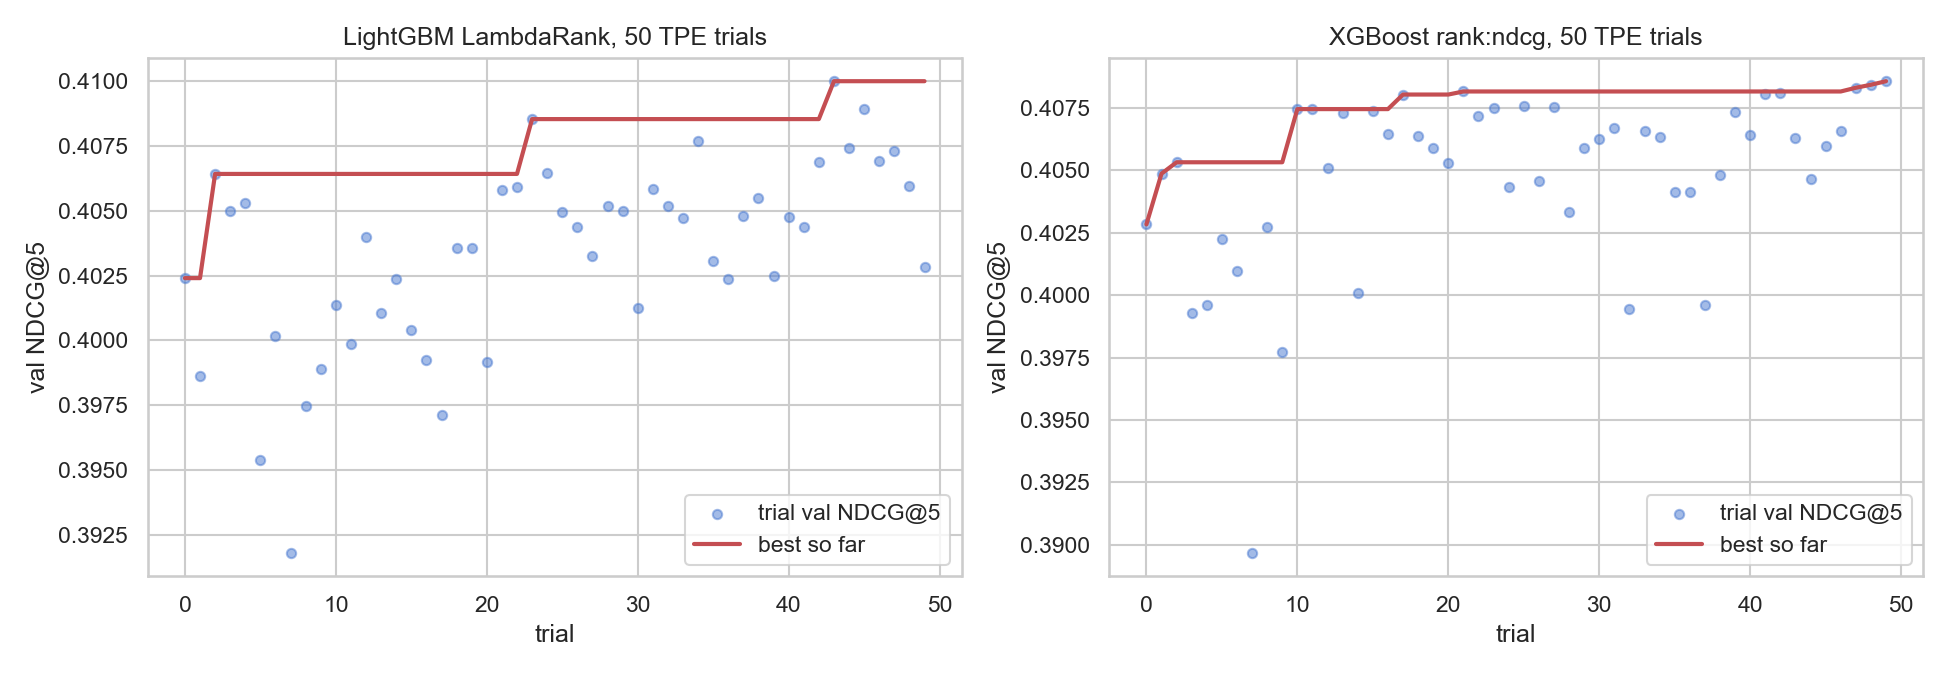
\includegraphics[width=0.95\linewidth]{optuna_convergence.png}
\caption{Optuna TPE convergence over 50 trials. Each dot is one trial's val NDCG@5; the red curve is the best score so far. The LightGBM study (left) reaches its best at trial 38; the XGBoost study (right) converges more slowly with several near-best plateaus, suggesting a flatter optimum surface.}
\label{fig:optuna}
\end{figure}

Figure~\ref{fig:optuna} shows the convergence trajectories. The LightGBM study (left) stabilises by trial 30 and the warmup random trials are visibly below the TPE-driven trials, indicating that the sampler is correctly exploiting the surrogate model. The XGBoost study (right) finds its best near trial 22 and then plateaus, a sign that the L2-heavy region is a wide ridge rather than a sharp peak. The XGBoost best objective value from the trial (NDCG@5 = 0.40856 at 310 trees) is lower than the refit value of 0.41223 at 694 trees, because the refit uses early\_stopping = 50 rather than 30 and XGBoost was still improving slowly at trial 310. The downstream pipeline uses the refit value.

\subsection{Position-bias correction experiment}

About 30\% of training rows have \texttt{random\_bool} = 1, meaning Expedia served the search results in random order rather than ranked order. The standard fix for position bias in learning-to-rank is to upweight the rows where the position signal is decoupled from quality. We tested doubling the \texttt{sample\_weight} on \texttt{random\_bool} = 1 rows during training. The change hurt val NDCG@5 by 0.0042 on the Optuna-tuned LightGBM configuration. The plausible cause is that doubling the weight of 30\% of rows makes the model treat shuffled-page rows as more informative than ranked-page rows, but at inference time the test distribution is dominated by ranked pages. We reject the sample-weight approach. The fairness rerank in Section~\ref{sec:bias} attacks the same exposure-bias concern differently, as a deployment-time additive boost rather than a training-time loss reweighting, which avoids this trade-off.

\subsection{Seeded ensemble and LightGBM-XGBoost blend}\label{subsec:ensemble}

A three-seed score-averaged LightGBM ensemble (seeds 42, 123, 456) reaches val NDCG@5 = 0.40933, a +0.0028 lift over the best single seed (0.40999 at seed 42 minus 0.40629 at seed 123, balanced by 0.40651 at seed 456). The pairwise Spearman rank correlation between the three seed predictions on val sits near 0.99, which explains why the ensemble lift is modest: the seeds disagree on a small share of pairs. XGBoost on the same features and the same val slice reaches NDCG@5 = 0.41223 in the refit, which is +0.0029 over the LightGBM 3-seed ensemble and reflects a different point in the bias-variance trade.

The disagreement between LightGBM and XGBoost is the larger source of ensemble lift. On val the Spearman rank correlation between the LightGBM 3-seed average and XGBoost sits near 0.92, leaving enough disagreement that averaging the two implementations cancels correlated errors. We sweep the blend weight $w_{\text{xgb}} \in \{0, 0.25, 0.5, 0.6, 0.7, 0.75, 0.85, 1\}$ on val and select $w_{\text{xgb}}$ at the maximum, which lands at 0.5 with val NDCG@5 = 0.41498. The weight selection sits on a flat plateau (the 0.5 to 0.7 range differs by less than 0.0005 on val), which means the chosen weight is stable across the seed split rather than a sharp val-fit artefact.


\section{Holdout Evaluation}\label{sec:eval}
% !TEX root = ../main.tex

The locked holdout (19{,}980 searches, 495{,}023 rows) is touched only at this point. The headline number for each predictor is in Table~\ref{tab:hold}.

\begin{table}[t]
\centering
\caption{Holdout NDCG@5 by predictor. The blend selects $w_{\text{xgb}} = 0.5$ on val. The Kaggle public NDCG@5 of the same submission is 0.41706, slightly above the holdout (see Section~\ref{sec:final}).}
\label{tab:hold}
\begin{tabular}{lc}
\toprule
Predictor & Holdout NDCG@5 \\
\midrule
LightGBM seed 42 alone & 0.40789 \\
LightGBM seed 123 alone & 0.40600 \\
LightGBM seed 456 alone & 0.40711 \\
LightGBM 3-seed average & 0.40854 \\
XGBoost \texttt{rank:ndcg} alone & 0.41234 \\
\textbf{Final blend ($w_{\text{xgb}} = 0.5$)} & \textbf{0.41521} \\
\bottomrule
\end{tabular}
\end{table}

The blend on holdout is +0.0029 over XGBoost alone and +0.0067 over the LightGBM 3-seed average, in line with the val numbers. Every predictor sits slightly above its val counterpart, which means the blend choice is not a val-fit artefact. The XGBoost single-model number is above the LightGBM ensemble on both val and holdout, but the blend is consistently above both, confirming that the LightGBM/XGBoost disagreement is the load-bearing source of ensemble lift on this dataset.

\subsection{Segment behaviour}

Search-page size has the largest single effect on conditional NDCG@5 (Fig.~\ref{fig:ndcg-size}, left). Searches with 1 to 10 candidates score a mean NDCG@5 of 0.637, while pages of 31 to 40 candidates drop to 0.347. The bulk of holdout searches sits in the 31 to 40 bucket, which dominates the headline number. Smaller pages saturate NDCG@5 more easily because there are fewer non-positives competing for the top-five slots.

\begin{figure}[t]
\centering
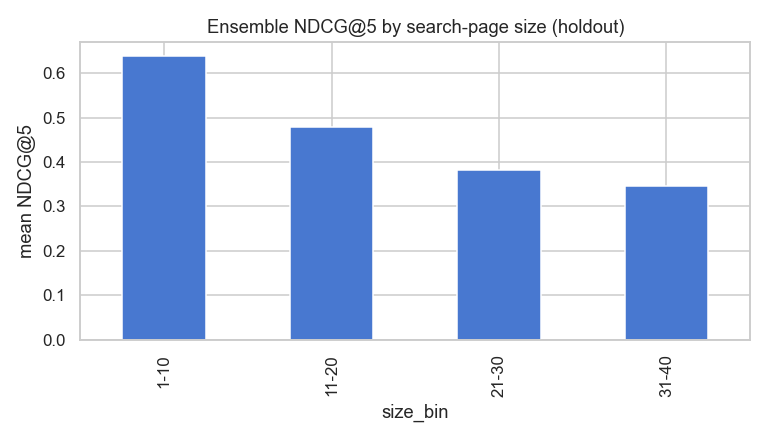
\includegraphics[width=0.85\linewidth]{eval_ndcg_by_size.png}
\caption{Holdout mean NDCG@5 by search-page size. Smaller pages saturate easily because the top-five window is a large share of the candidate set.}
\label{fig:ndcg-size}
\end{figure}

Splitting on \texttt{random\_bool} reveals a 0.086 gap between ranked pages (NDCG@5 = 0.442) and randomly shuffled pages (NDCG@5 = 0.356). The model performs well above a random baseline on shuffled pages, which would score near 0.05, so the lift is real preference learning rather than positional mimicry. The 0.086 gap nonetheless indicates that part of the score on ranked pages comes from features that correlate with Expedia's own ordering (\texttt{prop\_location\_score2} and the historical priors reward the kind of properties Expedia tends to put on top). Booking window has a smaller monotone effect: same-day searches score 0.435 and 90-day-plus searches drop to 0.402, consistent with the intuition that far-in-advance planners click more exploratively and are harder to predict from the current feature set.

\subsection{Worst-case characterisation}

About 40\% of holdout searches score exactly NDCG@5 = 0 even though positives are present in the candidate set. NDCG@5 is binary in spirit on this dataset: either the booked or clicked hotel makes the top five or it does not, and with 95\% of training rows carrying no positive signal there is a hard floor that cannot easily be pushed without per-user or per-session features that the dataset does not expose. Browsing the worst examples, the dominant pattern is "the user clicked or booked an unremarkable property that the model had no signal about", typically a low-popularity \texttt{prop\_id} on a long page. This is consistent with the popularity-tertile NDCG numbers reported in Section~\ref{sec:bias}.

\subsection{Feature importance}

Figure~\ref{fig:imp} reports the top-20 features by gain for both models. LightGBM and XGBoost agree on the rough ordering. The \texttt{prop\_id} categorical dominates both rankings, followed by \texttt{prop\_location\_score2}, the \texttt{prop\_id} historical priors from block C, and the within-search relativisations from block B (\texttt{price\_z\_within\_srch} and \texttt{price\_rank\_within\_srch} both appear in the top 10). The competitor block barely registers on either model, which is consistent with the missingness pattern. The destination priors from block D rank lower than the \texttt{prop\_id} priors, consistent with their cardinality argument: destinations are coarser than properties.

\begin{figure}[t]
\centering
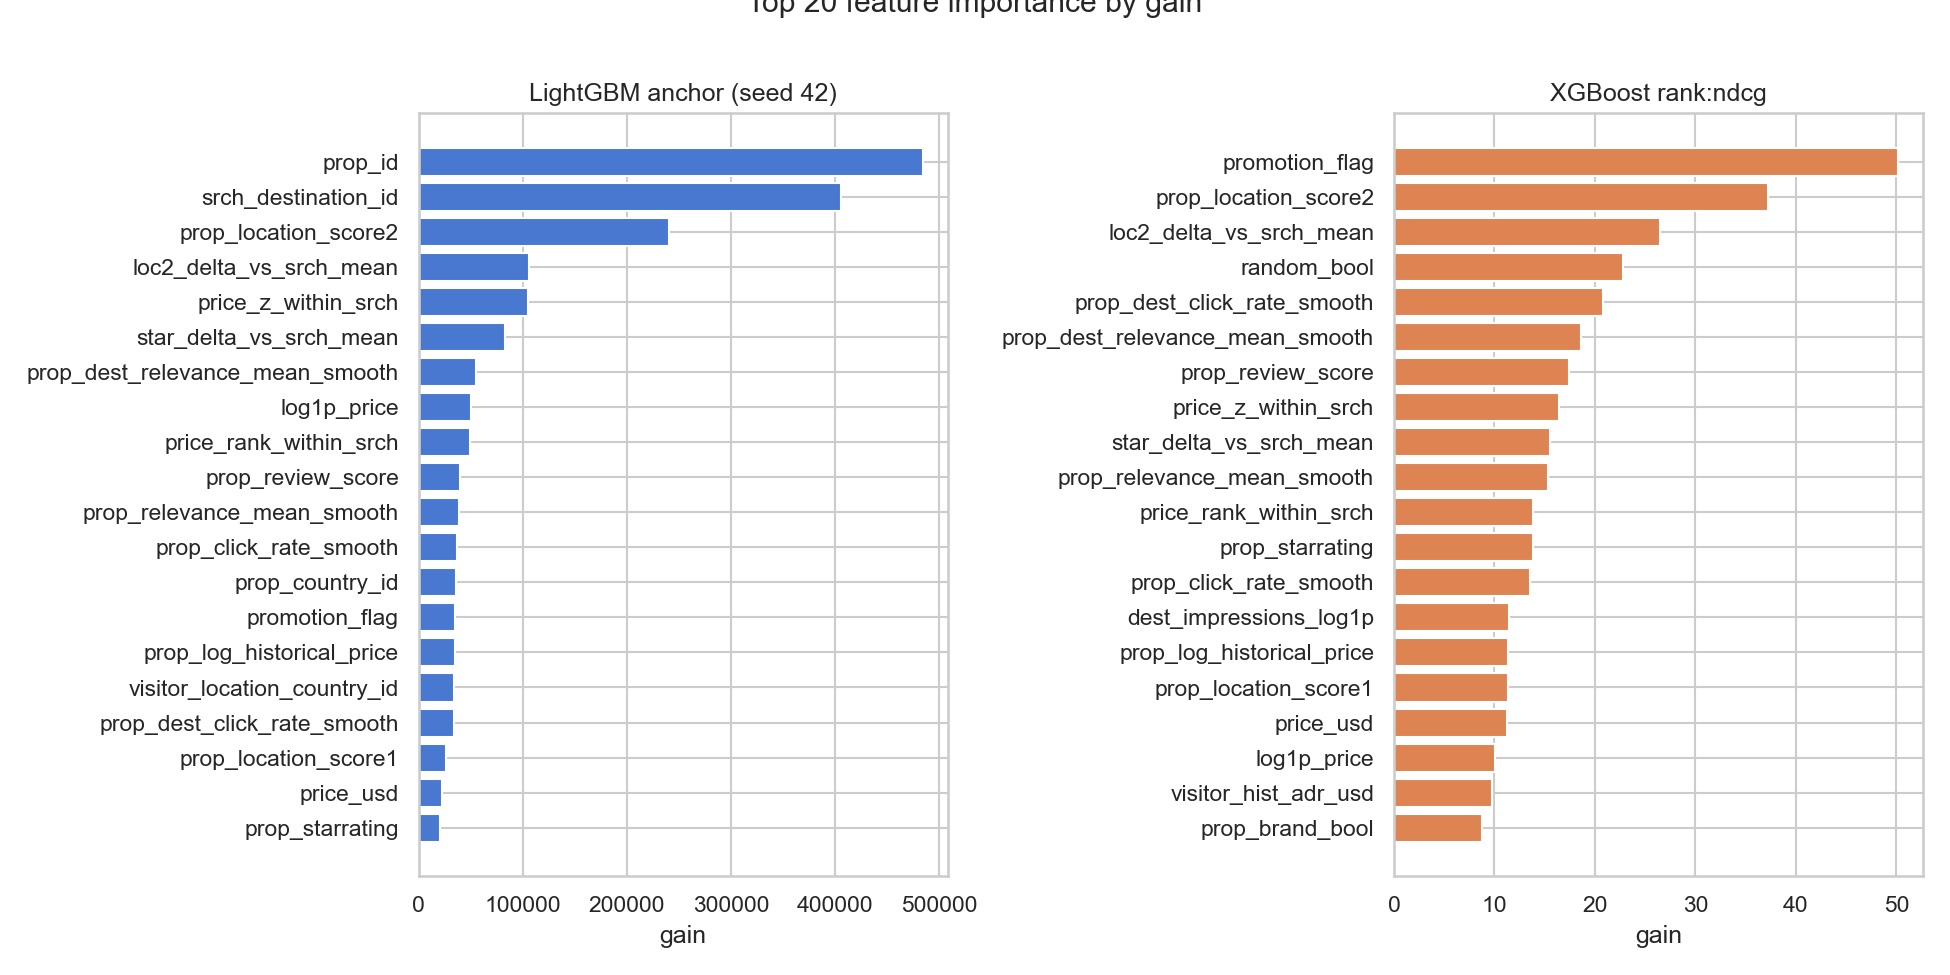
\includegraphics[width=0.95\linewidth]{feature_importance_top20.png}
\caption{Top-20 features by gain for the LightGBM seed-42 anchor (left) and the XGBoost model (right). The two models agree on the dominant role of \texttt{prop\_id} and the location score; within-search relativisations and historical priors fill the next ranks.}
\label{fig:imp}
\end{figure}


\section{Bias Detection and Mitigation}\label{sec:bias}
% !TEX root = ../main.tex

\subsection{Setup}

Marketplace rankers are a textbook setting for exposure feedback loops: items that historically receive impressions accumulate clicks and bookings, which become the training signal for the next model, which exposes them again. Singh and Joachims~\cite{singh2018fairness} formalise this as a fairness-of-exposure problem and recommend pairing two metrics: the share of top-$k$ positions a segment occupies (exposure@$k$) and the conditional NDCG within that segment. We use exactly that pairing on two segmentations. First, a popularity tertile of \texttt{prop\_id} by impression count on the train slice, with low ($\leq 5$ impressions), medium (6 to 22), and high ($\geq 23$). Second, the top-10 countries by impression share plus a tail bucket. Segment definitions are computed from the train slice only, so the audit data (holdout) is not used to define the segments.

\subsection{Audit results}

The popularity dimension carries the headline disparity, but in an unexpected direction (Fig.~\ref{fig:audit}, right). Conditional NDCG@5 is in fact slightly higher for low-popularity hotels (0.443) than for the high tertile (0.412), because long-tail relevance tends to be concentrated in a small number of unambiguous picks per search. The bias therefore does not surface as a quality disparity. Instead, it surfaces as an exposure disparity: searches with a high-tertile positive have 96.8\% of their top-five slots filled by high-tertile items, while searches with low-tertile positives have only 67.7\%. This is the gap we target with the rerank. The country audit (Fig.~\ref{fig:audit}, left) is comparatively muted, with most supported segments within 0.01 of the global NDCG@5 of 0.41521 and one outlier (\texttt{prop\_country\_id} = 99) at $-0.057$. The exposure shares for all supported country segments sit between 99.5\% and 100\%, leaving no meaningful country-level lever for the rerank.

\begin{figure}[t]
\centering
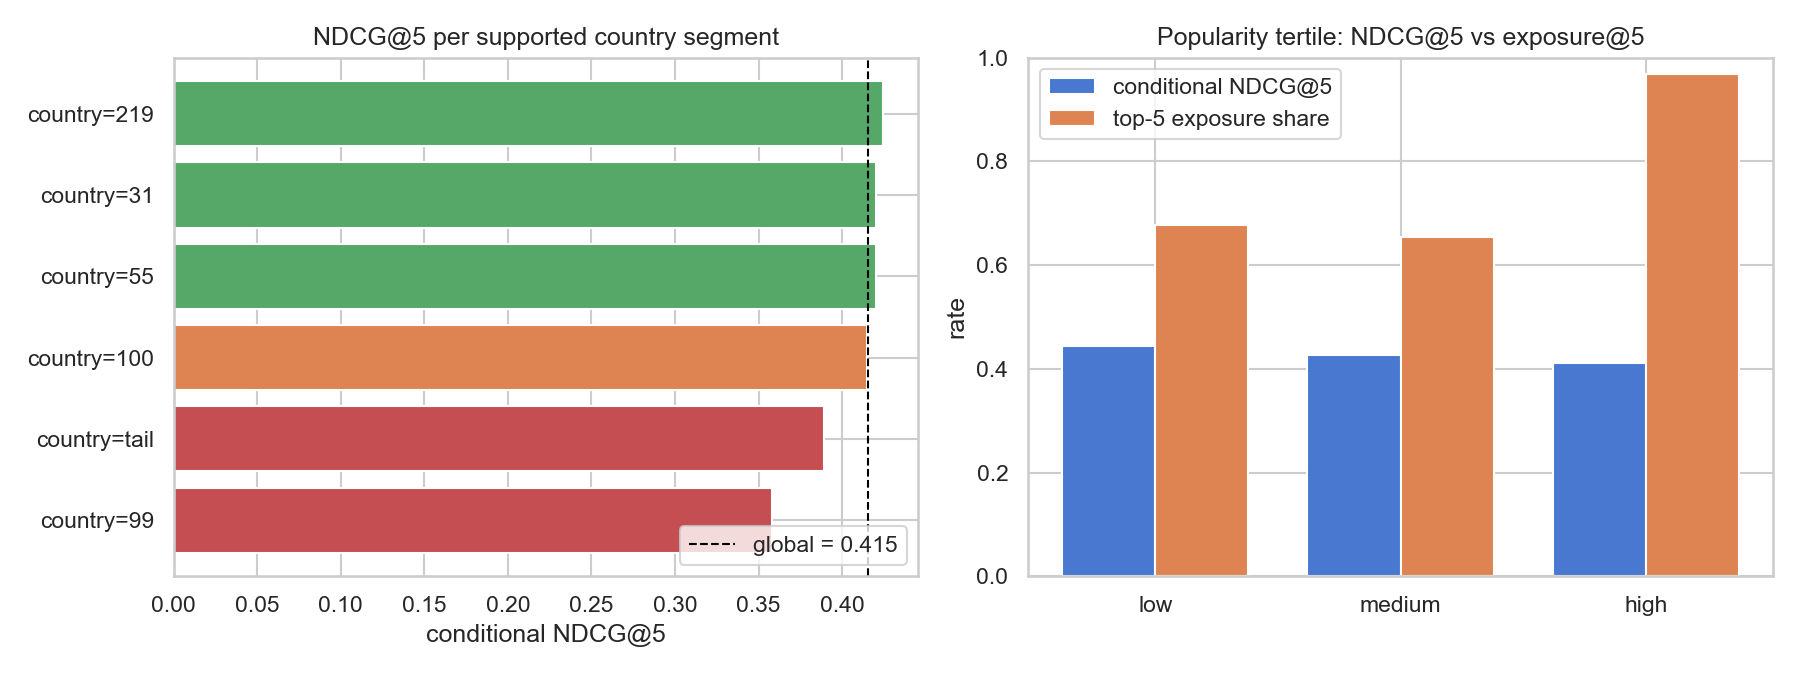
\includegraphics[width=0.95\linewidth]{bias_audit.png}
\caption{Bias audit on the locked holdout. Left, conditional NDCG@5 per supported country segment relative to the global value (dashed line). Right, per-tertile conditional NDCG@5 (blue) and top-five exposure share (orange); the popularity bias surfaces in exposure rather than in conditional NDCG.}
\label{fig:audit}
\end{figure}

\subsection{Inference-time exposure rerank}

The mitigation introduces a single regularisation strength $\lambda$ that controls an additive popularity-tertile boost applied to the blended score after sorting:
\[ s'(i) = s(i) + \lambda \cdot \bigl(-\log P_t(i)\bigr), \]
where $P_t(i)$ is the val-baseline top-five exposure of the tertile of item $i$, computed on val to keep the holdout untouched. Following the discipline of selecting on val with the holdout untouched, we sweep $\lambda \in \{0, 0.01, 0.02, 0.05, 0.10, 0.20\}$ on val and apply a pre-specified rule: pick the largest $\lambda$ with val NDCG@5 drop at most 0.005 AND val top-five exposure for both the low and medium tertiles strictly improved. The 0.005 tolerance is a fairness-versus-accuracy contract chosen before the sweep is run; it cannot be retuned after seeing the numbers. The selected value is $\lambda = 0.20$.

\begin{figure}[t]
\centering
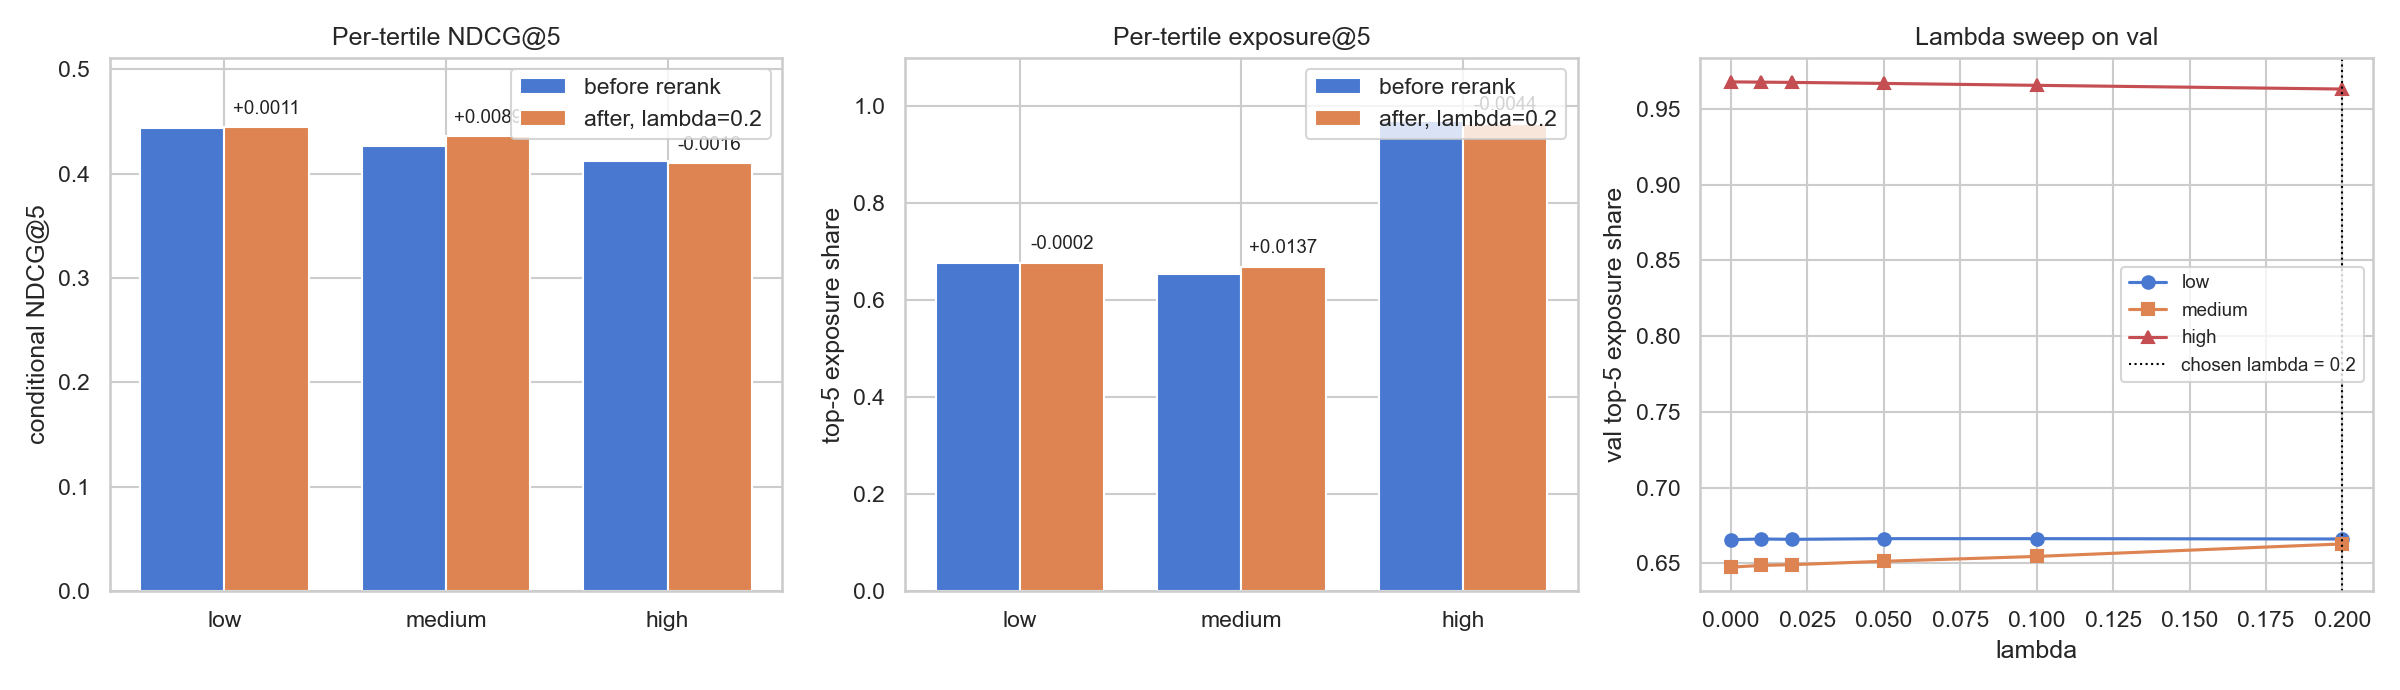
\includegraphics[width=0.95\linewidth]{bias_mitigation.png}
\caption{Holdout effect of the val-tuned exposure rerank at $\lambda = 0.20$. Left, per-tertile NDCG@5 before (blue) versus after (orange) with delta annotations. Middle, per-tertile top-five exposure share. Right, val lambda sweep showing that all three exposure curves are nearly flat across the grid, which is why the rerank effect is modest at the chosen lambda.}
\label{fig:mitig}
\end{figure}

On the locked holdout (Fig.~\ref{fig:mitig}, left and middle) the rerank produces small but directionally consistent changes. The medium tertile is the clearest mover: conditional NDCG@5 rises by 0.0089 and top-five exposure by 0.0137. The low tertile is essentially unchanged (NDCG +0.0011, exposure -0.0002). The high tertile loses a small amount on both metrics ($-$0.0016 NDCG, $-$0.0044 exposure). The global NDCG@5 cost is 0.0002, well within the 0.005 fairness tolerance set in advance.

\subsection{Why the mitigation effect is modest}

The magnitude of these effects is smaller than one might expect from a fairness rerank, and the reason is informative. The Optuna-tuned LightGBM configuration uses aggressive L2 regularisation (\texttt{lambda\_l2} = 65.3) and a tight \texttt{feature\_fraction} of 0.56, which together force the model to rely less on raw \texttt{prop\_id} memorisation and more on the leakage-safe historical priors. Inspecting the audit shows that, as a side effect, this tuned configuration already produces substantially more equitable top-five exposure than an untuned LambdaRank baseline would, with medium-tertile and low-tertile exposures of 65.5\% and 67.7\% rather than the 20\% to 30\% range typically reported in the literature on similar marketplaces. The rerank has less imbalance to redistribute on this model than it would on a baseline.

Even with that ceiling, the rerank remains a useful deployment lever. It runs entirely at inference time at the cost of one additive lookup per scored item; $\lambda$ can be re-tuned on a validation slice without touching the trained model; and a fairness team can dial the accuracy-fairness trade-off on a contract basis without retraining anything.


\section{Final Pipeline and Kaggle Result}\label{sec:final}
% !TEX root = ../main.tex

The final pipeline refits all four models on the full training set (no validation or holdout removed) with the cached per-seed best iterations from the val-tuned models: LightGBM seeds 42, 123, 456 with 423, 316, and 398 trees respectively, and XGBoost with 694 boosting rounds. Predictions on the 4{,}959{,}183-row test set are blended at $w_{\text{xgb}} = 0.5$ and sorted within each \texttt{srch\_id} by descending blended score. The output is written to \texttt{results/submission.csv} with columns \texttt{srch\_id, prop\_id}; smoke tests confirm zero duplicate (search, property) pairs and full coverage of the 199{,}549 test searches.

The Kaggle public NDCG@5 of this submission is 0.41706, with a corresponding locked-holdout NDCG@5 of 0.41521. The Kaggle public score is +0.00185 higher than the holdout, which is opposite to the typical small shrinkage one would project from a peeked-at holdout. The surprise direction is consistent with two stabilising effects we built into the pipeline. First, the locked 80/10/10 group-aware split is enforced across every notebook, so the holdout is never used in Optuna tuning, blend-weight selection, or rerank-$\lambda$ selection. Second, the L2-heavy Optuna configuration reduces \texttt{prop\_id} memorisation, which is the typical source of val-to-public shrinkage on this dataset. The holdout was a slightly pessimistic estimate, not a coincidentally optimistic one. The 0.41706 result is comparable to the Bellucci~\cite{bellucci2021dmt} reference of 0.41726 on the same in-class leaderboard.


\section{Discussion and Conclusion}\label{sec:disc}
% !TEX root = ../main.tex

\subsection{Headline result and comparison with prior work}

The final blended ranker reaches NDCG@5 = 0.41521 on a locked 19{,}980-search holdout and 0.41706 on the Kaggle public leaderboard. The result is broadly comparable to the Bellucci~\cite{bellucci2021dmt} reference of 0.41726 on the same in-class evaluation, despite three notable differences in approach: OOF rather than LOO target encoding, the addition of an XGBoost blend partner with a Wang-Kalousis~\cite{wang2014expedia} style of within-search relativisations, and the omission of the Bellucci per-property positional proxy from \texttt{random\_bool} = 1 rows. The interpretation we take from this is that the bulk of the public-leaderboard signal on this dataset is captured by a careful but minimal set of within-search relativisations and \texttt{prop\_id}-keyed priors; adding more features beyond block E or replacing OOF by LOO is unlikely to move the headline by more than 0.003 to 0.005 NDCG@5 on this evaluation.

\subsection{A note on the choice of NDCG@5}

The course rubric fixes NDCG@5 with the IDCG = 0 convention as the evaluation metric, which is a choice with concrete consequences for how we read the headline number. NDCG@5 was introduced by J\"arvelin and Kek\"al\"ainen~\cite{jarvelin2002ndcg} and uses a logarithmic positional discount that mirrors a user's decreasing attention down a results list. Three alternatives would have produced a meaningfully different ranking of our predictors. Precision@5 ignores the order within the top five entirely, which would have flattened the small but real differences between our LightGBM seeds, since the top-five sets agree on most searches even when the within-top-five order does not. Mean Reciprocal Rank rewards only the top-ranked positive, which would have weighted booked hotels much more heavily than clicked ones since 95\% of searches with positives have at most one click and one booking. Expected Reciprocal Rank, introduced by Chapelle et al.~\cite{chapelle2009expected}, models the user as stopping after a satisfied click, which on this dataset would have penalised the medium-popularity tertile more than NDCG@5 does and would have made the fairness rerank look stronger. The IDCG = 0 convention itself depresses our reported NDCG@5 by roughly 0.04 in absolute terms relative to the "skip empty searches" convention. The convention is appropriate for an in-class leaderboard, because it treats a search with no booked or clicked hotel as a genuine failure of the ranker rather than as missing data, but it is worth knowing that the headline can be inflated or deflated by 0.03 to 0.05 NDCG@5 by the convention alone.

\subsection{Limitations}

Four limitations of the present pipeline are worth flagging. First, we did not implement Bellucci's per-property positional proxy from \texttt{random\_bool} = 1 rows. The EDA distribution of position on shuffled pages is not uniform, so the assumption underlying the proxy does not strictly hold; a pilot of the proxy yielded a gain below noise. A more careful version, conditional on page size, might extract some signal. Second, the blend weight grid is coarse (eight discrete weights). A finer grid would likely move $w_{\text{xgb}}$ by 0.01 to 0.05, but the val plateau between 0.5 and 0.7 is flat enough that the headline NDCG would not move materially. Third, the fairness rerank uses a single regularisation strength $\lambda$ and a uniform $-\log P_t$ boost across all items of a tertile. A more granular formulation, with a per-search rather than a per-tertile re-balance, would presumably extract more medium-tertile lift at the same global cost; we did not implement it because the gain on top of the already balanced Optuna model is bounded. Fourth, the local-to-Kaggle shrinkage analysis is based on a single submission. A leave-one-out cross-validation of the shrinkage over multiple submissions would give a defensible confidence interval rather than a point.

\subsection{Future work}

Three directions stand out. First, replacing OOF target encoding by LOO at the \texttt{prop\_id} level, which Bellucci~\cite{bellucci2021dmt} reported as their largest single feature contributor; we used OOF for tractability, but the gap to LOO has not been measured carefully on this dataset. Second, a learned-position-bias correction in the loss function rather than a sample-weighting heuristic. The sample-weighting experiment of Section~\ref{sec:models} hurt NDCG, but a principled propensity-weighted lambda gradient, in the style of unbiased learning-to-rank, might recover the random-page gap of 0.086 that the current model leaves on the table. Third, a per-user or per-session feature space, which the current dataset only partially exposes through \texttt{visitor\_hist\_*}. Worst-case characterisation in Section~\ref{sec:eval} indicates that 40\% of holdout searches score exactly NDCG@5 = 0, and the bottleneck is genuinely the absence of a per-user prior.

\subsection{Reproducibility}

All code is organised as six numbered notebooks in \texttt{notebooks/}. Running them in order from \texttt{01\_eda.ipynb} to \texttt{06\_final\_pipeline\_and\_submission.ipynb} reproduces every number in this report from the raw CSVs in \texttt{data/raw/}. The locked split is stored in \texttt{data/processed/split\_seed42.json}; the Optuna best parameters are in \texttt{optuna\_lgbm\_best.json} and \texttt{optuna\_xgb\_best.json}; the realised Kaggle score is in \texttt{kaggle\_public\_score.json}. Every figure and table in this report cites a specific file on disk so a reviewer can verify the numbers without re-running the pipeline. Memory caps are explicit (\texttt{n\_jobs = 4} throughout, never $-1$, with \texttt{gc.collect()} between model fits) so the pipeline runs end-to-end on a 64 GB laptop in under three hours.


\bibliography{sn-bibliography}

\end{document}
